\documentclass[twoside]{article}

% Packages required by doxygen
\usepackage{fixltx2e}
\usepackage{calc}
\usepackage{doxygen}
\usepackage[export]{adjustbox} % also loads graphicx
\usepackage{graphicx}
\usepackage[utf8]{inputenc}
\usepackage{makeidx}
\usepackage{multicol}
\usepackage{multirow}
\PassOptionsToPackage{warn}{textcomp}
\usepackage{textcomp}
\usepackage[nointegrals]{wasysym}
\usepackage[table]{xcolor}

% NLS support packages
\usepackage{polski}
\usepackage[T1]{fontenc}

% Font selection
\usepackage[T1]{fontenc}
\usepackage[scaled=.90]{helvet}
\usepackage{courier}
\usepackage{amssymb}
\usepackage{sectsty}
\renewcommand{\familydefault}{\sfdefault}
\allsectionsfont{%
  \fontseries{bc}\selectfont%
  \color{darkgray}%
}
\renewcommand{\DoxyLabelFont}{%
  \fontseries{bc}\selectfont%
  \color{darkgray}%
}
\newcommand{\+}{\discretionary{\mbox{\scriptsize$\hookleftarrow$}}{}{}}

% Page & text layout
\usepackage{geometry}
\geometry{%
  a4paper,%
  top=2.5cm,%
  bottom=2.5cm,%
  left=2.5cm,%
  right=2.5cm%
}
\tolerance=750
\hfuzz=15pt
\hbadness=750
\setlength{\emergencystretch}{15pt}
\setlength{\parindent}{0cm}
\setlength{\parskip}{0.2cm}
\makeatletter
\renewcommand{\paragraph}{%
  \@startsection{paragraph}{4}{0ex}{-1.0ex}{1.0ex}{%
    \normalfont\normalsize\bfseries\SS@parafont%
  }%
}
\renewcommand{\subparagraph}{%
  \@startsection{subparagraph}{5}{0ex}{-1.0ex}{1.0ex}{%
    \normalfont\normalsize\bfseries\SS@subparafont%
  }%
}
\makeatother

% Headers & footers
\usepackage{fancyhdr}
\pagestyle{fancyplain}
\fancyhead[LE]{\fancyplain{}{\bfseries\thepage}}
\fancyhead[CE]{\fancyplain{}{}}
\fancyhead[RE]{\fancyplain{}{\bfseries\leftmark}}
\fancyhead[LO]{\fancyplain{}{\bfseries\rightmark}}
\fancyhead[CO]{\fancyplain{}{}}
\fancyhead[RO]{\fancyplain{}{\bfseries\thepage}}
\fancyfoot[LE]{\fancyplain{}{}}
\fancyfoot[CE]{\fancyplain{}{}}
\fancyfoot[RE]{\fancyplain{}{\bfseries\scriptsize Wygenerowano Śr, 15 kwi 2015 14\+:45\+:29 dla program framework benchmarkujacy dla abstrakcyjnego typu danych\+: tablica haszujaca. programem Doxygen }}
\fancyfoot[LO]{\fancyplain{}{\bfseries\scriptsize Wygenerowano Śr, 15 kwi 2015 14\+:45\+:29 dla program framework benchmarkujacy dla abstrakcyjnego typu danych\+: tablica haszujaca. programem Doxygen }}
\fancyfoot[CO]{\fancyplain{}{}}
\fancyfoot[RO]{\fancyplain{}{}}
\renewcommand{\footrulewidth}{0.4pt}
\renewcommand{\sectionmark}[1]{%
  \markright{\thesection\ #1}%
}

% Indices & bibliography
\usepackage{natbib}
\usepackage[titles]{tocloft}
\setcounter{tocdepth}{3}
\setcounter{secnumdepth}{5}
\makeindex

% Hyperlinks (required, but should be loaded last)
\usepackage{ifpdf}
\ifpdf
  \usepackage[pdftex,pagebackref=true]{hyperref}
\else
  \usepackage[ps2pdf,pagebackref=true]{hyperref}
\fi
\hypersetup{%
  colorlinks=true,%
  linkcolor=blue,%
  citecolor=blue,%
  unicode%
}

% Custom commands
\newcommand{\clearemptydoublepage}{%
  \newpage{\pagestyle{empty}\cleardoublepage}%
}


%===== C O N T E N T S =====

\begin{document}

% Titlepage & ToC
\hypersetup{pageanchor=false,
             bookmarks=true,
             bookmarksnumbered=true,
             pdfencoding=unicode
            }
\pagenumbering{roman}
\begin{titlepage}
\vspace*{7cm}
\begin{center}%
{\Large program framework benchmarkujacy dla abstrakcyjnego typu danych\+: tablica haszujaca. \\[1ex]\large 1.\+0 }\\
\vspace*{1cm}
{\large Wygenerowano przez Doxygen 1.8.9.1}\\
\vspace*{0.5cm}
{\small Śr, 15 kwi 2015 14:45:29}\\
\end{center}
\end{titlepage}
\tableofcontents
\pagenumbering{arabic}
\hypersetup{pageanchor=true}

%--- Begin generated contents ---
\section{program framework benchmarkujacy dla abstrakcyjnego typu danych\+: tablica haszujaca.}
\label{index}\hypertarget{index}{}\begin{DoxyAuthor}{Autor}
Wojciech Makuch 
\end{DoxyAuthor}
\begin{DoxyDate}{Data}
27.\+05.\+2015 
\end{DoxyDate}
\begin{DoxyVersion}{Wersja}
1.\+0
\end{DoxyVersion}
program testujacy oraz benchmarkujacy zaimplementowane grafy posiada menu uzytkownika do wyboru \hypertarget{index_utworz}{}\subsection{graf}\label{index_utworz}
\hypertarget{index_utworz}{}\subsection{graf}\label{index_utworz}
\hypertarget{index_wyswietl}{}\subsection{macierz sasiedztwa}\label{index_wyswietl}
\hypertarget{index_DSF}{}\subsection{D\+S\+F}\label{index_DSF}
\hypertarget{index_BFS}{}\subsection{B\+F\+S}\label{index_BFS}
\hypertarget{index_benchmarkuj}{}\subsection{D\+F\+Sa}\label{index_benchmarkuj}
\hypertarget{index_benchmarkuj}{}\subsection{D\+F\+Sa}\label{index_benchmarkuj}
\hypertarget{index_graf}{}\subsection{omawiany na cwiczeniach}\label{index_graf}
\hypertarget{main.cpp_wyjscie}{}\subsection{wyjscie}\label{main.cpp_wyjscie}

\section{Indeks klas}
\subsection{Lista klas}
Tutaj znajdują się klasy, struktury, unie i interfejsy wraz z ich krótkimi opisami\+:\begin{DoxyCompactList}
\item\contentsline{section}{\hyperlink{class_c_benchmark}{C\+Benchmark} }{\pageref{class_c_benchmark}}{}
\item\contentsline{section}{\hyperlink{class_c_edge}{C\+Edge} \\*Definicja klasy \hyperlink{class_c_edge}{C\+Edge} definuje krawedz grafu nie zawiera wag }{\pageref{class_c_edge}}{}
\item\contentsline{section}{\hyperlink{class_c_graph}{C\+Graph} \\*Definicja klasy \hyperlink{class_c_graph}{C\+Graph} definije graf skierowany bez wagowaych krawedzi dziedzicy po klasie \hyperlink{class_c_benchmark}{C\+Benchmark} }{\pageref{class_c_graph}}{}
\item\contentsline{section}{\hyperlink{class_c_node}{C\+Node} \\*Definicja klasy \hyperlink{class_c_node}{C\+Node} definiuje pojedynczy wezel grafu }{\pageref{class_c_node}}{}
\item\contentsline{section}{\hyperlink{classqueue}{queue} \\*Definicja klasy queue definicja kolejki A\+D\+T, kolejka typu F\+I\+F\+O zimplementowaa na liscie }{\pageref{classqueue}}{}
\item\contentsline{section}{\hyperlink{classqueue__node}{queue\+\_\+node} \\*Definicja klasy \hyperlink{classqueue__node}{queue\+\_\+node} definicja wezla dla kolejki definiuje pojedynczy element bedacy w kolejkce }{\pageref{classqueue__node}}{}
\end{DoxyCompactList}

\section{Indeks plików}
\subsection{Lista plików}
Tutaj znajduje się lista wszystkich plików z ich krótkimi opisami\+:\begin{DoxyCompactList}
\item\contentsline{section}{\hyperlink{format_8h}{format.\+h} }{\pageref{format_8h}}{}
\item\contentsline{section}{\hyperlink{global_8h}{global.\+h} }{\pageref{global_8h}}{}
\item\contentsline{section}{\hyperlink{graph_8cpp}{graph.\+cpp} \\*Implementuje zdefiniowana klase grafu }{\pageref{graph_8cpp}}{}
\item\contentsline{section}{\hyperlink{graph_8hh}{graph.\+hh} \\*Zwiera definicje klas \hyperlink{class_c_node}{C\+Node}, \hyperlink{class_c_edge}{C\+Edge}, C\+Grpah \hyperlink{class_c_node}{C\+Node} -\/ wezel grafu \hyperlink{class_c_edge}{C\+Edge} -\/ krawedz grafu \hyperlink{class_c_graph}{C\+Graph} -\/ graf }{\pageref{graph_8hh}}{}
\item\contentsline{section}{\hyperlink{main_8cpp}{main.\+cpp} }{\pageref{main_8cpp}}{}
\item\contentsline{section}{\hyperlink{queue_8cpp}{queue.\+cpp} \\*Implementuje zdefiniowana klase kolejki }{\pageref{queue_8cpp}}{}
\item\contentsline{section}{\hyperlink{queue_8hh}{queue.\+hh} \\*Zawiera definicje klas \hyperlink{classqueue__node}{queue\+\_\+node}, queue \hyperlink{classqueue__node}{queue\+\_\+node} -\/ wezel kolejki queue -\/ kolejka }{\pageref{queue_8hh}}{}
\item\contentsline{section}{\hyperlink{stack_8hh}{stack.\+hh} \\*Definicja struktury danych \hyperlink{class_lista}{Lista} }{\pageref{stack_8hh}}{}
\end{DoxyCompactList}

\section{Dokumentacja klas}
\hypertarget{classdane}{}\subsection{Dokumentacja klasy dane}
\label{classdane}\index{dane@{dane}}


{\ttfamily \#include $<$dane.\+hh$>$}

\subsubsection*{Metody publiczne}
\begin{DoxyCompactItemize}
\item 
char $\ast$ \hyperlink{classdane_a8fd41a54eb1cd6204e3ce1785ebb0413}{Wez\+Klucz} () const 
\begin{DoxyCompactList}\small\item\em definicja metody Wez\+Klucz klasy dane metoda nie pozwala na zmiane zawartosci pola. \end{DoxyCompactList}\item 
int \hyperlink{classdane_ad0fb107a74bafb30cff8bde81709403f}{Wez\+Wartosc} () const 
\begin{DoxyCompactList}\small\item\em definicja metody Wez\+Wartosc klasy dane. metoda nie pozwala na zmiane zawartosci pola. \end{DoxyCompactList}\item 
\hyperlink{classdane_a5cee48299360f96fe88622503a38e376}{dane} (char $\ast$k, int w)
\begin{DoxyCompactList}\small\item\em definicja konstruktora 2-\/parametrycznego \end{DoxyCompactList}\item 
\hyperlink{classdane_a680f7dc64c0fae8532539e51195fd2ff}{dane} ()
\begin{DoxyCompactList}\small\item\em definicja konstruktora bezparametrycznego zeruje pole wartosc, wskaznik na lancuch ustawia na N\+U\+L\+L \end{DoxyCompactList}\end{DoxyCompactItemize}


\subsubsection{Opis szczegółowy}


Definicja w linii 16 pliku dane.\+hh.



\subsubsection{Dokumentacja konstruktora i destruktora}
\hypertarget{classdane_a5cee48299360f96fe88622503a38e376}{}\index{dane@{dane}!dane@{dane}}
\index{dane@{dane}!dane@{dane}}
\paragraph[{dane}]{\setlength{\rightskip}{0pt plus 5cm}dane\+::dane (
\begin{DoxyParamCaption}
\item[{char $\ast$}]{k, }
\item[{int}]{w}
\end{DoxyParamCaption}
)\hspace{0.3cm}{\ttfamily [inline]}}\label{classdane_a5cee48299360f96fe88622503a38e376}


Definicja w linii 38 pliku dane.\+hh.

\hypertarget{classdane_a680f7dc64c0fae8532539e51195fd2ff}{}\index{dane@{dane}!dane@{dane}}
\index{dane@{dane}!dane@{dane}}
\paragraph[{dane}]{\setlength{\rightskip}{0pt plus 5cm}dane\+::dane (
\begin{DoxyParamCaption}
{}
\end{DoxyParamCaption}
)\hspace{0.3cm}{\ttfamily [inline]}}\label{classdane_a680f7dc64c0fae8532539e51195fd2ff}


Definicja w linii 44 pliku dane.\+hh.



\subsubsection{Dokumentacja funkcji składowych}
\hypertarget{classdane_a8fd41a54eb1cd6204e3ce1785ebb0413}{}\index{dane@{dane}!Wez\+Klucz@{Wez\+Klucz}}
\index{Wez\+Klucz@{Wez\+Klucz}!dane@{dane}}
\paragraph[{Wez\+Klucz}]{\setlength{\rightskip}{0pt plus 5cm}char$\ast$ dane\+::\+Wez\+Klucz (
\begin{DoxyParamCaption}
{}
\end{DoxyParamCaption}
) const\hspace{0.3cm}{\ttfamily [inline]}}\label{classdane_a8fd41a54eb1cd6204e3ce1785ebb0413}
\begin{DoxyReturn}{Zwraca}
pole prywane klucz. 
\end{DoxyReturn}


Definicja w linii 26 pliku dane.\+hh.

\hypertarget{classdane_ad0fb107a74bafb30cff8bde81709403f}{}\index{dane@{dane}!Wez\+Wartosc@{Wez\+Wartosc}}
\index{Wez\+Wartosc@{Wez\+Wartosc}!dane@{dane}}
\paragraph[{Wez\+Wartosc}]{\setlength{\rightskip}{0pt plus 5cm}int dane\+::\+Wez\+Wartosc (
\begin{DoxyParamCaption}
{}
\end{DoxyParamCaption}
) const\hspace{0.3cm}{\ttfamily [inline]}}\label{classdane_ad0fb107a74bafb30cff8bde81709403f}
\begin{DoxyReturn}{Zwraca}
pole prywatne wartosc 
\end{DoxyReturn}


Definicja w linii 33 pliku dane.\+hh.



Dokumentacja dla tej klasy została wygenerowana z pliku\+:\begin{DoxyCompactItemize}
\item 
\hyperlink{dane_8hh}{dane.\+hh}\end{DoxyCompactItemize}

\hypertarget{classtablica}{}\subsection{Dokumentacja klasy tablica}
\label{classtablica}\index{tablica@{tablica}}


definicja klasy tablica. Definiuje tablice haszujaca(asocjacyjna z mozliwoscia odwolania sie do jej elementu poprzez klucz). Tablica alokowana jest dynamicznie, rozmiar ustalany jest w konstruktorze. Tablica ma narzucony maksymalny rozmiar, poniewaz metoda haszujaca klucze na nim bazuje. Klasa zawiera 2 pola\+: tab -\/ tablice danych oraz zmienna rozmiar przechowujaca informacje o dlugosci tablicy.  




{\ttfamily \#include $<$haszowanie.\+hh$>$}

\subsubsection*{Metody publiczne}
\begin{DoxyCompactItemize}
\item 
\hyperlink{classtablica_a5ee1754d39209bec5987d4cbdf19f210}{tablica} (int n)
\begin{DoxyCompactList}\small\item\em definicja konstruktra 1-\/parametrowego \end{DoxyCompactList}\item 
\hyperlink{classtablica_a75c3c78102abf0e2b70652c174e02012}{$\sim$tablica} ()
\begin{DoxyCompactList}\small\item\em definicja destruktora \end{DoxyCompactList}\item 
\hyperlink{classdane}{dane} \hyperlink{classtablica_aaed9c2371e7f19d46dc0179995df529a}{operator\mbox{[}$\,$\mbox{]}} (int i) const 
\begin{DoxyCompactList}\small\item\em defiicja przeciazenia operatora \mbox{[}\mbox{]} \end{DoxyCompactList}\item 
\hyperlink{classdane}{dane} \hyperlink{classtablica_a8daad41788563f20b42a169da7f3d2fc}{operator\mbox{[}$\,$\mbox{]}} (char $\ast$klucz) const 
\begin{DoxyCompactList}\small\item\em definicja przeciazenia operatora \mbox{[}\mbox{]} pozwala na odwolanie sie do elementu tablicy za pomoca klucza \end{DoxyCompactList}\item 
int \hyperlink{classtablica_a4ea08247dfa3fc56630be6cde3bfa3e1}{Haszowanie} (char $\ast$klucz) const 
\begin{DoxyCompactList}\small\item\em definicja metody Haszowanie pierszy sposob haszowania klucza dodaje elementu klucza zrzutowane na inta, liczy reszte z dzielenia przez maksymalny rozmiar metoda nie zmienia stanu obiektu \end{DoxyCompactList}\item 
int \hyperlink{classtablica_aa87cd29bc045e60e19ccf374112723e2}{Drugie\+Haszowanie} (char $\ast$klucz) const 
\begin{DoxyCompactList}\small\item\em definicja metody Drugie\+Haszowanie drugi sposob haszowania klucza. wykorzystuje wzor 1-\/(dodany wartosci klucza)/q, gdzie q jest polowa maksymalnego rozmiaru i q jest liczba nieparzysta. metoda nie zmienia stanu obiektu. Drugie\+Haszowanie wykorzystuje sie w celu zminimalizowania ilosci wystapien kolizji. \end{DoxyCompactList}\item 
void \hyperlink{classtablica_a85187198b332fe2cc899166cba2fc9aa}{Wypelnij} (\hyperlink{classdane}{dane} element)
\begin{DoxyCompactList}\small\item\em definicja metody Wypelnij Ustawia element w tablicy haszowania zgodnie z wartoscia klucza Jezeli dojdzie do 1. kolizji, zostaje wykorzystane drugie haszowanie i sprawdzana jest dostepnosc komorki i+j, gdzie i-\/wynik pierwszego haszowania, j -\/ wynik drugiego haszowania. Jezeli dochodzi do kolejnych kolizji tablica zostaje wypelniana poprzez przechodzenie z komorki do komorki o 1 dalej. \end{DoxyCompactList}\item 
void \hyperlink{classtablica_a8a6c216f7c281127ea2d8820bacb8431}{Wyswietl} () const 
\begin{DoxyCompactList}\small\item\em definicja metody Wyswietl metoda pomocna przy tworzeniu programu. Wypisuje na strumien wyjsciowy zawartosc tablicy, przy odwolaniu sie do wartosci elementow(a nie do kluczy). Metoda nie zmienia stanu obiektu. \end{DoxyCompactList}\end{DoxyCompactItemize}


\subsubsection{Opis szczegółowy}


Definicja w linii 19 pliku haszowanie.\+hh.



\subsubsection{Dokumentacja konstruktora i destruktora}
\hypertarget{classtablica_a5ee1754d39209bec5987d4cbdf19f210}{}\index{tablica@{tablica}!tablica@{tablica}}
\index{tablica@{tablica}!tablica@{tablica}}
\paragraph[{tablica}]{\setlength{\rightskip}{0pt plus 5cm}tablica\+::tablica (
\begin{DoxyParamCaption}
\item[{int}]{n}
\end{DoxyParamCaption}
)}\label{classtablica_a5ee1754d39209bec5987d4cbdf19f210}


Definicja w linii 4 pliku haszowanie.\+cpp.

\hypertarget{classtablica_a75c3c78102abf0e2b70652c174e02012}{}\index{tablica@{tablica}!````~tablica@{$\sim$tablica}}
\index{````~tablica@{$\sim$tablica}!tablica@{tablica}}
\paragraph[{$\sim$tablica}]{\setlength{\rightskip}{0pt plus 5cm}tablica\+::$\sim$tablica (
\begin{DoxyParamCaption}
{}
\end{DoxyParamCaption}
)}\label{classtablica_a75c3c78102abf0e2b70652c174e02012}


Definicja w linii 10 pliku haszowanie.\+cpp.



\subsubsection{Dokumentacja funkcji składowych}
\hypertarget{classtablica_aa87cd29bc045e60e19ccf374112723e2}{}\index{tablica@{tablica}!Drugie\+Haszowanie@{Drugie\+Haszowanie}}
\index{Drugie\+Haszowanie@{Drugie\+Haszowanie}!tablica@{tablica}}
\paragraph[{Drugie\+Haszowanie}]{\setlength{\rightskip}{0pt plus 5cm}int tablica\+::\+Drugie\+Haszowanie (
\begin{DoxyParamCaption}
\item[{char $\ast$}]{klucz}
\end{DoxyParamCaption}
) const}\label{classtablica_aa87cd29bc045e60e19ccf374112723e2}

\begin{DoxyParams}{Parametry}
{\em \mbox{[}klucz\mbox{]}} & zadany klucz \\
\hline
\end{DoxyParams}
\begin{DoxyReturn}{Zwraca}
kod bedacy wynikiem drugiego haszowania 
\end{DoxyReturn}


Definicja w linii 34 pliku haszowanie.\+cpp.

\hypertarget{classtablica_a4ea08247dfa3fc56630be6cde3bfa3e1}{}\index{tablica@{tablica}!Haszowanie@{Haszowanie}}
\index{Haszowanie@{Haszowanie}!tablica@{tablica}}
\paragraph[{Haszowanie}]{\setlength{\rightskip}{0pt plus 5cm}int tablica\+::\+Haszowanie (
\begin{DoxyParamCaption}
\item[{char $\ast$}]{klucz}
\end{DoxyParamCaption}
) const}\label{classtablica_a4ea08247dfa3fc56630be6cde3bfa3e1}

\begin{DoxyParams}{Parametry}
{\em \mbox{[}klucz\mbox{]}} & zadany klucz \\
\hline
\end{DoxyParams}
\begin{DoxyReturn}{Zwraca}
kod bedacy wnikiem pierwszego haszowania 
\end{DoxyReturn}


Definicja w linii 15 pliku haszowanie.\+cpp.

\hypertarget{classtablica_aaed9c2371e7f19d46dc0179995df529a}{}\index{tablica@{tablica}!operator\mbox{[}$\,$\mbox{]}@{operator[]}}
\index{operator\mbox{[}$\,$\mbox{]}@{operator[]}!tablica@{tablica}}
\paragraph[{operator[]}]{\setlength{\rightskip}{0pt plus 5cm}{\bf dane} tablica\+::operator\mbox{[}$\,$\mbox{]} (
\begin{DoxyParamCaption}
\item[{int}]{i}
\end{DoxyParamCaption}
) const\hspace{0.3cm}{\ttfamily [inline]}}\label{classtablica_aaed9c2371e7f19d46dc0179995df529a}

\begin{DoxyParams}{Parametry}
{\em \mbox{[}i\mbox{]}} & komorka tablicy pozwala na odwolanie sie do elementu tablicy o indeksie i metoda nie pozwala na zmiane wartosci pol prywatnych \\
\hline
\end{DoxyParams}
\begin{DoxyReturn}{Zwraca}
element tablicy 
\end{DoxyReturn}


Definicja w linii 41 pliku haszowanie.\+hh.

\hypertarget{classtablica_a8daad41788563f20b42a169da7f3d2fc}{}\index{tablica@{tablica}!operator\mbox{[}$\,$\mbox{]}@{operator[]}}
\index{operator\mbox{[}$\,$\mbox{]}@{operator[]}!tablica@{tablica}}
\paragraph[{operator[]}]{\setlength{\rightskip}{0pt plus 5cm}{\bf dane} tablica\+::operator\mbox{[}$\,$\mbox{]} (
\begin{DoxyParamCaption}
\item[{char $\ast$}]{klucz}
\end{DoxyParamCaption}
) const}\label{classtablica_a8daad41788563f20b42a169da7f3d2fc}

\begin{DoxyParams}{Parametry}
{\em \mbox{[}klucz\mbox{]}} & zadany klucz \\
\hline
\end{DoxyParams}
\begin{DoxyReturn}{Zwraca}
element tablicy 
\end{DoxyReturn}


Definicja w linii 96 pliku haszowanie.\+cpp.

\hypertarget{classtablica_a85187198b332fe2cc899166cba2fc9aa}{}\index{tablica@{tablica}!Wypelnij@{Wypelnij}}
\index{Wypelnij@{Wypelnij}!tablica@{tablica}}
\paragraph[{Wypelnij}]{\setlength{\rightskip}{0pt plus 5cm}void tablica\+::\+Wypelnij (
\begin{DoxyParamCaption}
\item[{{\bf dane}}]{element}
\end{DoxyParamCaption}
)}\label{classtablica_a85187198b332fe2cc899166cba2fc9aa}
w 
\begin{DoxyParams}{Parametry}
{\em \mbox{[}element\mbox{]}} & dane przekazywane do tablicy \\
\hline
\end{DoxyParams}


Definicja w linii 57 pliku haszowanie.\+cpp.

\hypertarget{classtablica_a8a6c216f7c281127ea2d8820bacb8431}{}\index{tablica@{tablica}!Wyswietl@{Wyswietl}}
\index{Wyswietl@{Wyswietl}!tablica@{tablica}}
\paragraph[{Wyswietl}]{\setlength{\rightskip}{0pt plus 5cm}void tablica\+::\+Wyswietl (
\begin{DoxyParamCaption}
{}
\end{DoxyParamCaption}
) const}\label{classtablica_a8a6c216f7c281127ea2d8820bacb8431}


Definicja w linii 87 pliku haszowanie.\+cpp.



Dokumentacja dla tej klasy została wygenerowana z plików\+:\begin{DoxyCompactItemize}
\item 
\hyperlink{haszowanie_8hh}{haszowanie.\+hh}\item 
\hyperlink{haszowanie_8cpp}{haszowanie.\+cpp}\end{DoxyCompactItemize}

\section{Dokumentacja plików}
\hypertarget{benchmark_8cpp}{}\subsection{Dokumentacja pliku benchmark.\+cpp}
\label{benchmark_8cpp}\index{benchmark.\+cpp@{benchmark.\+cpp}}
{\ttfamily \#include \char`\"{}benchmark.\+hh\char`\"{}}\\*
{\ttfamily \#include $<$windows.\+h$>$}\\*
{\ttfamily \#include $<$fstream$>$}\\*
{\ttfamily \#include $<$iostream$>$}\\*

\hypertarget{benchmark_8hh}{}\subsection{Dokumentacja pliku benchmark.\+hh}
\label{benchmark_8hh}\index{benchmark.\+hh@{benchmark.\+hh}}
{\ttfamily \#include $<$windows.\+h$>$}\\*
\subsubsection*{Komponenty}
\begin{DoxyCompactItemize}
\item 
class \hyperlink{class_c_benchmark}{C\+Benchmark}
\end{DoxyCompactItemize}

\hypertarget{dane_8hh}{}\subsection{Dokumentacja pliku dane.\+hh}
\label{dane_8hh}\index{dane.\+hh@{dane.\+hh}}


plik przechowujacy deklaracje klasy dane oraz deklaracje jej pol i metod.  


\subsubsection*{Komponenty}
\begin{DoxyCompactItemize}
\item 
class \hyperlink{classdane}{dane}
\end{DoxyCompactItemize}


\subsubsection{Opis szczegółowy}
/$\ast$! definicja klasy dane. Jest to struktura przechowujaca klucz poddawany haszowaniu oraz wartosc jako przechowywane dane (zmienna typu int). Obiekty typu dane sa wykorzystywane do wypelniania tablicy haszujacej(asocjacyjnej). Pole klucz mozna potraktowac np. jako nazwisko szukanej osoby w bazie danych, a pole wartosc jako jej nr telefonu. Klasa zawiera metody pozwalajace na odwolanie sie do pol prywatnych bez nadpisywania ich oraz konstruktory. 
\hypertarget{haszowanie_8cpp}{}\subsection{Dokumentacja pliku haszowanie.\+cpp}
\label{haszowanie_8cpp}\index{haszowanie.\+cpp@{haszowanie.\+cpp}}
{\ttfamily \#include $<$iostream$>$}\\*
{\ttfamily \#include \char`\"{}haszowanie.\+hh\char`\"{}}\\*

\hypertarget{haszowanie_8hh}{}\subsection{Dokumentacja pliku haszowanie.\+hh}
\label{haszowanie_8hh}\index{haszowanie.\+hh@{haszowanie.\+hh}}


plik przechowyjacy deklaracje klasy tablica oraz deklaracje jej pol i metod.  


{\ttfamily \#include \char`\"{}dane.\+hh\char`\"{}}\\*
\subsubsection*{Komponenty}
\begin{DoxyCompactItemize}
\item 
class \hyperlink{classtablica}{tablica}
\begin{DoxyCompactList}\small\item\em definicja klasy tablica. Definiuje tablice haszujaca(asocjacyjna z mozliwoscia odwolania sie do jej elementu poprzez klucz). Tablica alokowana jest dynamicznie, rozmiar ustalany jest w konstruktorze. Tablica ma narzucony maksymalny rozmiar, poniewaz metoda haszujaca klucze na nim bazuje. Klasa zawiera 2 pola\+: tab -\/ tablice danych oraz zmienna rozmiar przechowujaca informacje o dlugosci tablicy. \end{DoxyCompactList}\end{DoxyCompactItemize}

\hypertarget{losowy__lancuch_8hh}{}\subsection{Dokumentacja pliku losowy\+\_\+lancuch.\+hh}
\label{losowy__lancuch_8hh}\index{losowy\+\_\+lancuch.\+hh@{losowy\+\_\+lancuch.\+hh}}


plik przechowujacy fukncje do zwracania losowych lancuchow  


{\ttfamily \#include $<$cstdlib$>$}\\*
\subsubsection*{Funkcje}
\begin{DoxyCompactItemize}
\item 
char \hyperlink{losowy__lancuch_8hh_a694ee1735eb83c733c781ca0fe1e39d8}{Losowy\+Znak} ()
\begin{DoxyCompactList}\small\item\em definicja funkcji Losowy\+Znak Funkcja inline. \end{DoxyCompactList}\item 
char $\ast$ \hyperlink{losowy__lancuch_8hh_ae5ce74a76ccb659a022323f5d4783492}{Losowy\+Lancuch} ()
\begin{DoxyCompactList}\small\item\em definicja funkcji Losowy\+Lancuch Metoda inline. \end{DoxyCompactList}\end{DoxyCompactItemize}


\subsubsection{Dokumentacja funkcji}
\hypertarget{losowy__lancuch_8hh_ae5ce74a76ccb659a022323f5d4783492}{}\index{losowy\+\_\+lancuch.\+hh@{losowy\+\_\+lancuch.\+hh}!Losowy\+Lancuch@{Losowy\+Lancuch}}
\index{Losowy\+Lancuch@{Losowy\+Lancuch}!losowy\+\_\+lancuch.\+hh@{losowy\+\_\+lancuch.\+hh}}
\paragraph[{Losowy\+Lancuch}]{\setlength{\rightskip}{0pt plus 5cm}char$\ast$ Losowy\+Lancuch (
\begin{DoxyParamCaption}
{}
\end{DoxyParamCaption}
)\hspace{0.3cm}{\ttfamily [inline]}}\label{losowy__lancuch_8hh_ae5ce74a76ccb659a022323f5d4783492}
\begin{DoxyReturn}{Zwraca}
losowy lancuch znakow o dlugosci od 0 do 10. 
\end{DoxyReturn}


Definicja w linii 25 pliku losowy\+\_\+lancuch.\+hh.

\hypertarget{losowy__lancuch_8hh_a694ee1735eb83c733c781ca0fe1e39d8}{}\index{losowy\+\_\+lancuch.\+hh@{losowy\+\_\+lancuch.\+hh}!Losowy\+Znak@{Losowy\+Znak}}
\index{Losowy\+Znak@{Losowy\+Znak}!losowy\+\_\+lancuch.\+hh@{losowy\+\_\+lancuch.\+hh}}
\paragraph[{Losowy\+Znak}]{\setlength{\rightskip}{0pt plus 5cm}char Losowy\+Znak (
\begin{DoxyParamCaption}
{}
\end{DoxyParamCaption}
)\hspace{0.3cm}{\ttfamily [inline]}}\label{losowy__lancuch_8hh_a694ee1735eb83c733c781ca0fe1e39d8}
\begin{DoxyReturn}{Zwraca}
wartosc liczbowa znaku A\+S\+C\+I\+I z przedzialu od A do Z. 
\end{DoxyReturn}


Definicja w linii 15 pliku losowy\+\_\+lancuch.\+hh.


\hypertarget{main_8cpp}{}\subsection{Dokumentacja pliku main.\+cpp}
\label{main_8cpp}\index{main.\+cpp@{main.\+cpp}}
{\ttfamily \#include $<$iostream$>$}\\*
{\ttfamily \#include $<$cstdlib$>$}\\*
{\ttfamily \#include \char`\"{}losowy\+\_\+lancuch.\+hh\char`\"{}}\\*
{\ttfamily \#include \char`\"{}haszowanie.\+hh\char`\"{}}\\*
{\ttfamily \#include \char`\"{}dane.\+hh\char`\"{}}\\*
{\ttfamily \#include \char`\"{}benchmark.\+hh\char`\"{}}\\*
{\ttfamily \#include $<$ctime$>$}\\*
{\ttfamily \#include $<$fstream$>$}\\*
\subsubsection*{Funkcje}
\begin{DoxyCompactItemize}
\item 
int \hyperlink{main_8cpp_ae66f6b31b5ad750f1fe042a706a4e3d4}{main} ()
\end{DoxyCompactItemize}


\subsubsection{Dokumentacja funkcji}
\hypertarget{main_8cpp_ae66f6b31b5ad750f1fe042a706a4e3d4}{}\index{main.\+cpp@{main.\+cpp}!main@{main}}
\index{main@{main}!main.\+cpp@{main.\+cpp}}
\paragraph[{main}]{\setlength{\rightskip}{0pt plus 5cm}int main (
\begin{DoxyParamCaption}
{}
\end{DoxyParamCaption}
)}\label{main_8cpp_ae66f6b31b5ad750f1fe042a706a4e3d4}


Definicja w linii 26 pliku main.\+cpp.




\title{Laboratorium 5 - Sprawozdanie}
\author{Wojciech Makuch}


\maketitle
\section{Zadanie}
Program framework benchmarkujacy dla zaimplementowanego abstrakcyjnego typu danych: tablica haszujaca.
\section{Realizacja}
Program wykonano na bazie zwyklej tablicy alokowanej dynamicznie o zadanym maksymalnym rozmiarze. Rozmiar nie może byc zmienny, ponieważ metody haszujace bazują na operacji dzielenia modulo przez ten rozmiar, jego zmiana spowodowałaby znaczne pogorszenie złożoności obliczeniowej. Program zwiera 2 struktury: pierwsza przechowuje dane(element, wartość), druga to tablica przechowujaca te dane. Program zawiera 2 metody haszujace. Pierwsza z nich bazuje na operacji dzielenia modulo przez maksymalny rozmiar wartosci liczbowej kodu ASCII klucza. Druga metoda wykorzystuje wzor q-(dodany wartosci klucza)/q, gdzie q jest polowa maksymalnego rozmiaru i q jest liczba nieparzysta. Zasada wypelniania tablicy jest nastepujaca:
\begin{enumerate}
	\item WezKlucz
	\item i$\leftarrow$ PierwszeHaszowanie
	\item jeśli tab[i]=0, to wypełnij komórke. \\
	w przypadku przeciwnym:
	\item $j\leftarrow$ DrugieHaszowanie
	\item jeśli tab[i+j]=0, to wypełnij komórkę. \\
	w przypadku przeciwnym:
	\item Wypelnij najblizsza wolno komorkę.
\end{enumerate}
Ponadto program zawiera przeciązenie operatora [] pozwalającego odnieść się do wybranej komórki tablicy haszującej(asocjacyjnej) za pomocą klucza. Algorytm działa na tym samym schemacie, co wypłenianie.
\section{Działanie}
Program tak samo jak poprzednie nie udostępnia użytkownikowi interfesju. Po uruchomieniu jedynie wyswietla dane, które są jednocześnie zapisywane do pliku o nazwie \textsl{pomiar\_czas\_5.txt}. Główna funkcja programu wywołuje jednynie funkcje \textsl{benchmarkuj()}, która zawiera pętle zliczania i zpaisywania uzyskanych wyników.

\section{Wyniki}
Przetestowano czas wypełniania tablicy haszującej elementami losowymi. Uzyskane dane przedstawiono na rys 1. Wynika z nich wprost, że złożoność obliczeniowa wynosi $O(n^{2})$, lecz po aproksymacji widać, ze współczynik przy $x^{2}$ jest bardzo mały(0.0046), co oznacza, że wykres mozna również przyblizyć prostą. Wtedy złożoność obliczeniowa wyniesie $O(n)$. jest to najgorszy możliwy przypadek szukania pustej komórki przechodząc się kolejno po elementach tablicy, co dzieje się dosyć często przy wypełnianiu tablicy tak duzą ilocią elementów. Na rys 2. pokazano ten sam wykres dla mneijszej ilosci danych, Widać tu, że żadna funkcja nie jest ani rosnąca, ani malejąca. Może to sugerować złożoność obliczeniową O(1) dla małej ilości elementów.
\begin{figure}[h!]
\centering
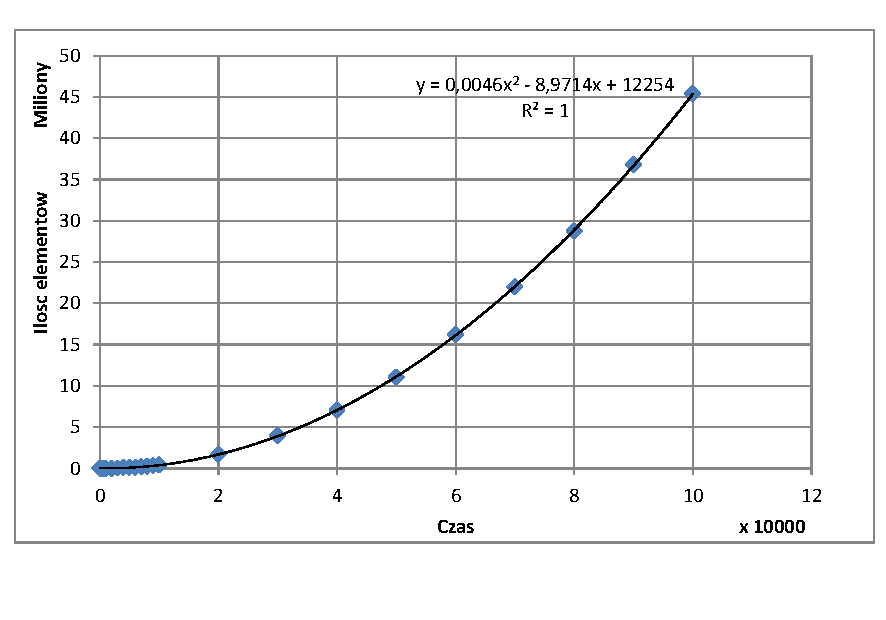
\includegraphics[scale=0.75]{Wykres1.pdf}
\caption{Wykres złożoności obliczeniowej dla dużej ilości elementów.}
\label{fig:wykres1}
\end{figure}
\begin{figure}[h!]
	\centering
	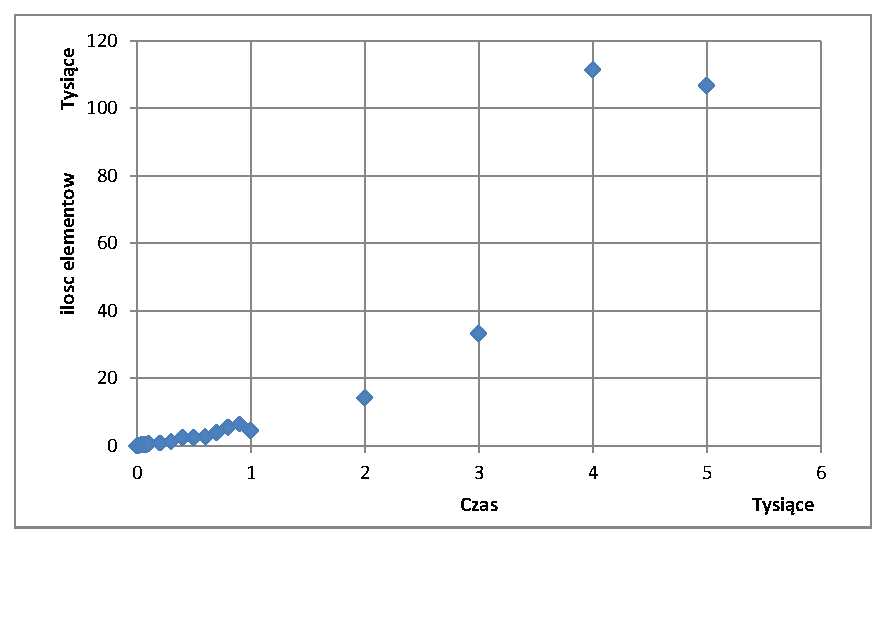
\includegraphics[scale=0.75]{Wykres2.pdf}
	\caption{Wykres złożoności obliczeniowej dla małej ilości elementów}
	\label{fig:wykres2}
\end{figure}
\section{Podsumowanie}
Złozoność obliczeniowa algorytmu wypełniania tablicy haszującej w najgorszym przypadku dla dużej ilości elementów jest $O(n)$ lub $O(n^{2})$ natomiast w najlepszym przypadku dla małej ilości jest $O(1)$.
\section{Komentarz}
Do utworzenia dokumentacji wykorzystano system Doxygen.
Funkcja pomiaru czasu dla systemu Windows pobrana ze strony dr. J. Mierzwy. Program skompilowano w środowisku Code::Blocks. Do stworzonia wykresu posłużono się pakietem MS Excel, sprawozdanie napisano używając systemu \LaTeX.
\end{document}